\newpage
\chapter{Workflow Builder}

\begin{figure}[h]
	\centering
	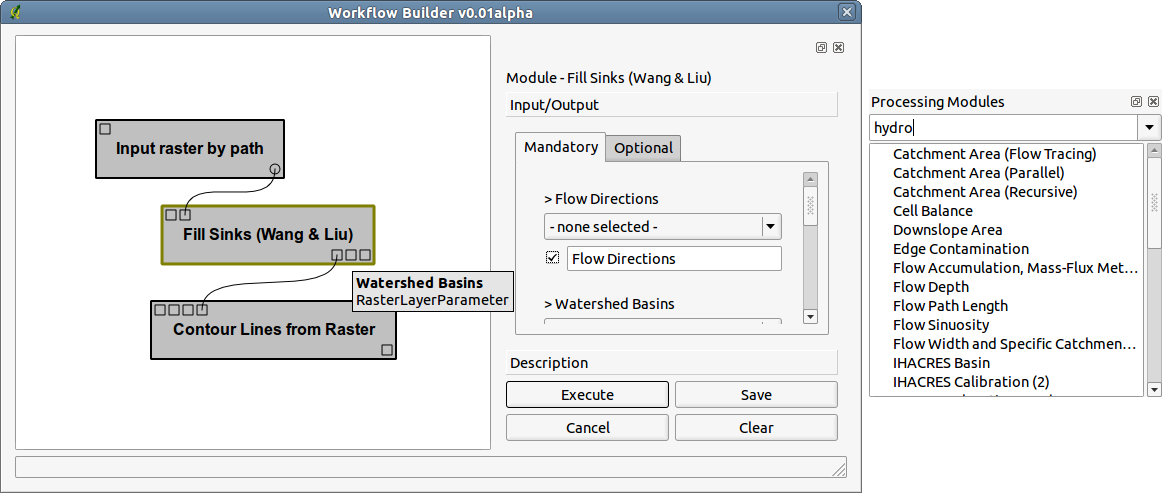
\includegraphics[scale=0.38]{pictures/wf/wf_pm}
	\caption{Workflow Builder}
  	\label{wf}
\end{figure}

Workflow Builder umožňuje uživateli propojovat moduly z QGIS Processing Framework. Výsledný graf lze poté jednoduše uložit jako nový modul QGIS Processing Frameworku. Dialogové okno Workflow Builder se skládá ze scény v levé části, která slouží k manipulaci s moduly, jejich propojování pomocí myši. V panelu v pravá části lze zadávat jednotlivé parametry modulů, které nejsou propojeny. V pravé spodní části se nachází tlačítka pro spuštění a uložení procesu, pro smazání scény a pro vypnutí dialogového okna. Jakmile uživatel klikne na tlačítko pro uložení, otevře se nové dialogové okno, kde bude vyzván k nastavení nového modulu. Jméno modulu, tagy, popis a hlavně parametry. U parametrů může uživatel nastavit, zdali chce, aby se parametr musel zadávat pokaždé i v novém modulu, či hodnota bude pokaždé stejná a tudíž se nemusí ani zobrazovat. Dále může uživatel nastavit alternativní název parametru.

Pro práci s Workflow Builder je dobré mít také alespoň jeden plugin, který registruje své moduly v QGIS Processing Frameworku, dále plugin \textbf{Workflow for Processing Framework Manager}, který byl napsán pro načítání modulů vytvořených pomocí Workflow Builderu a uložených ve formátu XML. Dále se může hodit \textbf{Input parameters for WB}, který přidává do Processing Frameworku moduly, které slouží pro načítání vektorových a rastrových dat se souboru.

\noindent Pro začátek můžete shlédnout instruktážní video: 
\begin{center}
	\href{http://youtu.be/4PxvWvTIyaU}{\texttt{http://youtu.be/4PxvWvTIyaU}}
\end{center}


\section{Tvorba workflow}
Při spuštění Workflow Builderu se vytvoří objekt Graph. Do něho se postupně přidávají či z něj mažou moduly (třídy Module) a spojení (třídy Connection). Při přetažení PF Modulu do scény se vytvoří modul Module, který se uloží do Graphu. Modul obsahuje parametry PF Moduly, které jsou reprezentovány třídou Port. Grafická reprezentace Module je QGraphicsModule, který také podle Portů v Module vytvoří QGraphicsPort. Při spojování portů mezi sebou se kontroluje, zdali koresponduje typ (RasterLayerParameter, NumericPrameter, ...), spojuje-li se vstupní parametr s výstupním, zdali nejsou oba parametry parametry stejného modulu a pokud je vstupní parametr prázdný (to znamená, že není spojený s jiným parametrem). Pakliže jsou splněny všechny podmínky, vytvoří se spojení třídy Connection a jeho grafická reprezentace QGraphicsConnection. Connection se poté přidá do Graphu. Pro tvorbu spojení stačí kliknout na požadovaný vstup/výstup a táhnout myší na druhý parametr.

V Graphu máme tedy uloženy moduly a spojení mezi nimi (Module a Connetion). Jsou uloženy jako slovníky - id:Module, resp. id:Connection. Ty se během tvorby mění jak uživatel přidává a odebírá moduly, spojuje je a maže spojení. Zrušit modulu či spojení můžeme tím, že si jej myší označíme a stiskneme klávesu \textit{Delete}. 

\section{Spuštění procesu}
Jakmile se uživatel rozhodne spustit celý proces (workflow) začíná se tvořit graf. 

Tvoří se rekurzivně tak, že ze se vytvoří podgraf třídy SubGraph, z prvotního seznamu všech modulů v grafu se vyjme jeden a vloží se de něj. Poté se vyjmou z původního seznamu všechny moduly spojené s prvním modulem a vkládají se podgrafu, poté se z původního seznamu vyjmou moduly, které jsou spojené s předchozími moduly a tak dále dokud existují spojení. Zároveň se ukládají do podgrafu i spojení. Pakliže již neexistuje další propojený modul a v původním seznamu ještě zůstali nějaké moduly, vytvoří se nový podgraf a postupuje se stejně jako u předchozího. Jakmile nezůstali žádné moduly v seznamu, začneme postupně spouštět workflow.

Postupně se spouští každý podgraf. První se kontroluje zdali jsou u jeho modulů nastaveny všechny povinné vstupní parametry, případně jestli u nich existuje spojení. Pakliže se narazí na modul, u kterého není nějaký modul nastaven, uloží se do seznamu nevalidních modulů. Jakmile se projdou všechny moduly v podgrafu všechny jsou v pořádku, začne se s {\color{red} kontrolou, zdali podgraf neobsahuje smyčku}. Jeli stále vše v pořádku začneme s rekurzivním spouštění modulů. Pakliže nejsou všechnu moduly v pořádku, zastaví se provádění procesu spuštění a označí se moduly, které je třeba ještě nastavit, a ve spodní liště Module Builderu se vypíše poznámka, že je třeba označené moduly nastavit. Pakliže podgraf obsahuje smyčku, proces se také zastaví a také vypíše poznámku na spodní liště.

Obrázek se smyčkou

Obrázek se s nenastavenými moduly

Zde bych chtěl podotknou 

{\color{red} pseudokód rekurzivní ho spouštění modulů}

Pozn. kontrolují se pouze vstupní parametry, protože SAGA Plugin momentálně ignoruje zdali nastavíme výstupní parametr či ne; vytvoří si vždy nový

\section{Uložení workflow}
XML soubor se uloží do \$$HOME/.qgis/python/workflows$. 
\subsection{Popsání výstupního xml souboru}
XML nabízí jednoduché uložení hierarchicky strukturovaný dat. O prvcích XML dokumentu hovoříme jako elementech. Elementy jsou ohraničeny počátečními a koncovými značkami, tzv. tagy. XML dokument obsahuje vždy právě jeden kořenový element. Ten se může skládat z dalších a dalších elementů. V našem případě je kořenový element Graph. Ten se skládá z minimálně jednoho podgrafu (SubGraph), a ten poté minimálně z jednoho modulu (Module). Podgraf dále může obsahovat spojení mezi moduly (Connection). Modul kromě toho obsahuje elementy parametr (Port) a tag (tag) a popis. Graf také obsahuje tagy a popis. 

\begin{table}	
	\centering
	\begin{tabular}{|c|c|}
		\hline
		atribut & příklad \\
		\hline
		name & Addition two rasters \\
		tags & ['raster', 'hydrology'] \\	
		\hline	
	\end{tabular}
	\caption{atributy elementu Graph}
	\label{tab:graph}
\end{table}

\section{Načtení workflow do PF Manageru}
